\chapter[Benchmark orodja]{Benchmark orodja}

\pagestyle{fancy}
\fancyhf{}
\fancyhead[LE,RO]{\thepage}
\fancyhead[RE,LO]{\leftmark}

\huge Žiga Šebenik, Tomaž Mrežar
\normalsize
\bigskip

\section{Opis problema}
Na voljo je več brezplačnih benchmark orodij za določanje zmogljivosti računalniških sistemov. V tem poglavju bomo našteli najbolj uporabljena brezplačna orodja v praksi.
Vsako orodje bova opisala in naštela njihove prepoznavne značilnosti in prednosti pred drugimi.
  


\section{Benchmark orodja}
Obstaja več vrst benchmark orodij. Testi, ki jih benchmark orodja izvajajo se lahko razlikujejo med seboj vendar so osnovne funkcionalnosti testov skoraj povsod enake. Skorajda vsako orodje testira dosegljivost sistemov, upočasnitve delovanja, latenco sistema in prepustnost sistema. Orodja bova delila na dve skupini, prva skupina bodo orodja, ki so brezplačna, medtem ko bodo v drugo skupino spadala orodja, ki so plačljiva, brezplačna za končen čas ali pa imajo v brezplačni verziji omejene funkcionalnosti.

\section{Brezplačna orodja}
Brezplačno orodje je:
\begin{itemize}
\item Ročno benchmark testiranje
\item PerfKit Benchmarker
\end{itemize}

\subsection{Ročno benchmark testiranje}
Zelo preprosta izbira, ki nam je na voljo, je da preprosto sami testiramo zmogljivost oblačnih storitev s pomočjo več različnih orodij, vsako namenjeno specifičnemu delu sistema. Na voljo nam je veliko zastonjskih orodij, precej jih je tudi odprtokodnih, znani med njimi pa so: ping, Geekbench, fio, iPerf... Testiramo lahko zmogljivost posameznega strežnika, gruče ali pa celotnega oblaka. Njihova prednost je, da so preprosta in fleksibilna, vendar pa moramo več dela opraviti sami.

\subsection{PerfKit Benchmarker}
PerfKit Benchmarker je odprto kodno orodje uporabljeno za meriti in primerjati oblačne performanse.
Podpira več večjih oblačnih ponudnikov, kot so:
\begin{itemize}
\item Google Cloud Platform
\item Amazon Web Services
\end{itemize}
in tudi mnoge druge. PerfKit Benchmarker meri končni čas za zagotavljanje virov v oblaku in tudi vse osnovne oblačne meritve naštete v zgornjem poglavju. PerfKit Benchmarker zmanjšuje kompleksnost v zaganjanju testov na oblačnih ponudnikih z enotnimi in preprostimi ukazi.
Vsebuje tudi množice javnih testov za uporabo. Vsi testi se zaženejo z privzeto konfiguracijo, ki ni nastavljena v prid nobenemu ponudniku oblačnih storitev. To ponuja možnost testiranja na več različnih oblačnih platformah.

\section{Plačljiva orodja}
Plačljiva orodja so:
\begin{itemize}
\item SPEC Cloud® IaaS 2018
\item Cloud Spectator
\item Cloud Performance Benchmark
\item Technology Business Research, Inc.
\end{itemize}

\subsection{SPEC Cloud® IaaS 2018}

SPEC Cloud® IaaS 2018 testira delovanje infrastrukture kot storitev oblačnih implementacij. Podpira testiranje javnih in zasebnih oblakov. Orodje deluje nad strežbo storitve, kot tudi nad izvajanjem storitve oblaka z uporabo vhodno izhodnih in CPE intenzivnih del. Vsako delo se zažene kot distribuirana aplikacija narejena iz 6 ali 7 instanc, ki obremenijo oblakove resource (CPE, diski in omrežje). Delo bo teklo dokler testi ne naredijo več kakovosti storitve. Administrator lahko tudi omeji število aplikacij kreiranih med izvedbo.
Orodje nam omogoča obremeniti računsko zmogljivost, shrambo in omrežje oblaka. Pri tem pa ne potrebuje hypervizorja ali virtualizacijske plasti in uporablja delovne obremenitve, ki spominjajo na tiste, ki običajno delujejo v oblaku, kot so aplikacije za socialne medije in velika analiza podatkov.

\subsection{Cloud Spectator}

Cloud Spectator sicer ni orodje, ampak podjetje, ki ponuja benchmarking in konzultacijo glede oblačnih storitev. Podjetjem pomaga z analizo različnih ponudnikov oblačnih storitev in testira zmogljivost njihove infrastrukture ter svetuje pri ekonomskih odločitvah. Namenjen je tako primerjavi ponudnikov oblačnih storitev, kot tudi ponudnikom samim, da lahko analizirajo zmogljivost svoje infrastrukture. Nudili naj bi sposobnost izbire pravega ponudnika, kjer stranka postavi zahteve svoje aplikacije, Cloud spectator pa s kombinacijo zahtevosti strankine aplikacije, zmogljivosti infrastrukture različnih ponudnikov in njihovih cenikov, izbere pravega ponudnika.


\subsection{Cloud Performance Benchmark}

Cloud Performance Benchmark je poročilo o največjih petih ponudnikih Amazon Web Services, Google Cloud Platform, Microsoft Azure, IBM Cloud in Alibaba Cloud. Zagotavljalo naj bi nepristransko strokovno poročilo, ki je podprto z raznimi metrikami. Poročilo primerja infrastrukturo posameznega ponudnika in pokaže kako ta infrastruktura vpliva na zmogljivost ter jih seveda primerja med seboj. Prav tako se dotakne geografskih razlik in njihov vpliv na zmogljivost.

\subsection{Technology Business Research, Inc.}

Technology Business Research, Inc. je podjetje, ki prav tako nudi storitve tako ponudnikom oblačnih storitev, kot tudi njihovim strankam. Ponudnikom nudijo podatke o trgu, finančne podatke o ponudnikih programske opreme, napovedi, strategije prodaje, itd. Poslužnikom oblačnih storitev pa nudijo podatke o ponudnikih le teh storitev, zmogljivosti ponudnikove infrastrukture za strankin primer uporabe ter tudi prihajajoče trende, ki se bodo posluževali in vplivali na zmogljivost oblačnih sistemov.



%||||||||||||||||||||||||||||| EXAMPLI ||||||||||||||||||||||||||||||||||||||||||||||||||||||||||||||||||||||||||||||||||||||||||
\section{Tehnična navodila za pisanje teksta}
Seminarsko nalogo v obliki pričujočega poglavja napišite v \LaTeX okolju.

Na vire se sklicujte z zapisom \cite{1_dOcean}, \cite{1_greenwade93}. Slike uvrščajte v tekst na naslednji način. Na sliki \ref{fig:1_osnovnaShema} je predstavljen primer storitve, pri čemer morajo biti vse slike v EPS formatu.
\begin{figure}[H]
    \centering
    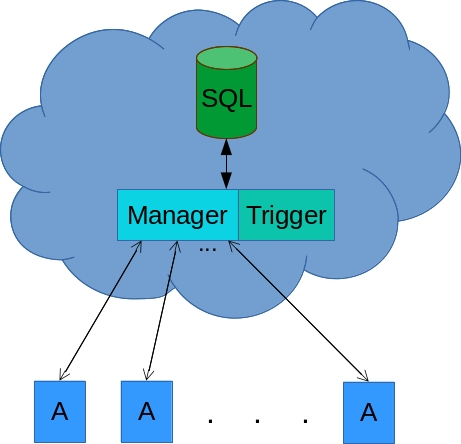
\includegraphics[scale=0.75]{Img/1_shema.jpg}
    \caption{Primer vstavitve slike v vaše poročilo.}
    \label{fig:1_osnovnaShema}
\end{figure}

Alineje naštevamo po naslednjem vzorcu:
\begin{itemize}
\item procesor: 1 jedro, Intel Xeon CPU E5-2650L v3 @ 1.8GHz,
\item ram: 1GB,
\item disk: 30GB.
\end{itemize}


V tabeli \ref{table:1_chunks} je prikazanih nekaj podatkov.
\begin{table}[H]
    \centering
        \begin{tabular}{ | r | r | r | r |} 
            \hline
           velikost koščkov & \textit{x} & \textit{y} & \textit{z} \\
            \hline
            Google Drive & 10 MB & 5 MB & 15 MB \\
            Mega & 1 MB & 0.5 MB & 1.5 MB \\
            \hline
        \end{tabular}
        \caption{Privzeta velikost koščkov \textit{x}, polovična privzeta velikost \textit{y} in za polovico povečana privzeta velikost \textit{z}.}
    \label{table:1_chunks}
\end{table}

Koda je predstavljena v izpisu \ref{lst:1_lst_cpu}.
\begin{lstlisting}[caption={Primer testiranja procesorja.}, label={lst:1_lst_cpu}]
zzrs@ZZRS:~$ sysbench --test=cpu --cpu-max-prime=20000 run
sysbench 0.4.12:  multi-threaded system evaluation benchmark

Running the test with following options:
Number of threads: 1

Doing CPU performance benchmark

Threads started!
Done.

Maximum prime number checked in CPU test: 20000


Test execution summary:
    total time:                          29.6635s
    total number of events:              10000
    total time taken by event execution: 29.6616
    per-request statistics:
         min:                                  2.55ms
         avg:                                  2.97ms
         max:                                 56.83ms
         approx.  95 percentile:               3.33ms

Threads fairness:
    events (avg/stddev):           10000.0000/0.00
    execution time (avg/stddev):   29.6616/0.00
\end{lstlisting}


\section{Zaključek}
Tule bo zaključek.

